\documentclass[twoside]{protokoll}
\usepackage{graphicx}
\usepackage{tabularx} % for better table formatting
\usepackage{booktabs} % for better table formatting
\usepackage{float} 
\praktikum{I}
\usepackage{subfig}
\usepackage{amsmath}

\versuchsgebiet{(E-Lehre)}


\teilnehmer{Maximilian Carlos Menke, 434170}
\teilnehmer{Andrea Roth, 428396}
\gruppe{A3}

\begin{document}
 
\section{1E3 Gekoppelte LC-Schwingkreise}

\begin{aufgabe}{Grundlagen}
  Knappe Beschreibung der theoretischen Grundlagen, Angabe der
  benötigten Formel(n), ohne Herleitung. Definition der verwendeten
  Formelzeichen.
\end{aufgabe}

\begin{aufgabe}{Versuchsaufbau und Versuchsdurchführung}
  Beschreibung des Versuchsaufbaus einschließlich
  Schaltbild. Beschreibung der Versuchsdurchführung: verwendete
  Messwerterfassungseinstellungen, Messbereiche, Triggerbedingungen,
  etc.
\end{aufgabe}

\subsection{Kurze Zusammenfassung des Aufbaus und Durchführung}

Detaillierter Aufbau und Durchführung zu den einzelnen Versuchsteilen, finden Sie am Anfang von den jeweiligen Abschnitten. 
Hier soll der Gesamtversuch kurz Dargestellt werden.\\

Der Versuch besteht aus insgesamt 3 Teilen. Für den ersten Teilversuch haben wir zwei LC-Schwingkreise Aufgebaut mit gleichen Bauteilen und die Schwingung in diesen einzeln gemessen. 
Diese sind Schwingkreise mit je einem Kondensator und einer Spule.
Als Widerstand in der Schaltung liegt nur der Innenwiederstand von Spule und Kondensator und den Kabeln vor. 
An den Schwingkreis wird eine Spannungsquelle angeschlossen, welche mithilfe eines Tasters kurzgeschlossen werden kann und den Schwingkreis schließt. 
Der Spannungsverlauf wird über dem Kondensator parallel gemessen. 
Dieser Teilversuch dient dazu den Einzelschwingkreis zu charakterisieren, dies wird Später benötigt zur Auswertung der gekoppelten Schwingkreise.\\

Zur Kopplung der Schwingkreise werden die Spulen nebeneinander gestellt und auch die Spannung am zweiten Kondensator gemessen. Durch drücken des Tasters wird eine Messung gestartet.
Als Einflussfaktoren auf den Kopplungsgrad wird das Variieren des Abstands der Spulen untersucht und der Einfluss eines Eisenkerns\\

Im letzten Teilversuch werden nun beide Kondensatoren mit der gleichen Spannungsquelle geladen. 
So, dass der Strom ein mal gleich sinnig durch die Spulen läuft und ein mal gegen sinnig. Die Schwingungen haben wir wieder an beiden Kondensatoren gemessen, und daraus die Frequenzen $f_+$ und $f_-$ bestimmt. 
 

\begin{aufgabe}{Vorversuch: Charakterisierung der verwendeten Bauteile}
  Charakterisieren Sie die verwendeten Bauteile mit Digitalvoltmeter
  bzw. Messbrücke.
\end{aufgabe}

Vor der Durchführung der Versuche, und zum späteren Vergleich der Messungen mit unseren Erwartungen haben wir die Bauteile charakterisiert. Dies haben wir mit einer Messbrücke getan. 

\begin{figure}[H]
    \centering
    \includegraphics[width=0.8\textwidth]{bilder/Messbrücke_10Ohm.pdf}
    \caption{Charakterisierung des 10 $\mu F$ Kondensator}
\end{figure}

In dem Bild zu sehen ist die Messbrücke, an die Stelle wo der Kondensator ist, wir das Bauteil angeschlossen. Das Bild ist noch mit unserem ersten Kondensator, diesen haben wir im Verlauf des Experiments gegen einen kleineren ausgetauscht, und alle Messungen mit dem kleineren wiederholt.\\

Für die Messung haben wir unseren Frequenzbereich von 1kHz eingestellt.
 (In dem Bild auf 100Hz weil wir da noch den 10 $\mu F$ messen, und wir mit diesem geringere Frequenzen hatten.) 
 Die Spulle haben wir ebenfalls gemessen wenn diese einen Eisenkern hatten, um den Einfluss von diesem auf Widerstand und Induktivität zu bestimmen.
So konnten wie sämtliche Bauteile Charakterisieren und sind für unseren zweiten Aufbau (mit kleinerem Kondensator) zu folgenden Ergebnissen gekommen:\\
    
\begin{table}[H]
        \centering
        \begin{tabularx}{0.8\textwidth}{X l c} % adjust width as needed
            \toprule
            \textbf{Bauteil} & \textbf{Messung} & \textbf{Fehler} \\
            \midrule
            Spule 1 & R = 2.344 $\Omega$ \quad L = 9.023mH &  \\
            mit Eisenkern & R = 2.70 $\Omega$ \quad L = 55.79mH & \\
            \midrule
            Spule 2 & R = 2.423 $\Omega$ \quad L = 8.981mH &  \\
            mit Eisenkern & R = 2.65 $\Omega$ \quad L = 56.1mH&\\
            \midrule
            Kondensator 1 & 2.301 $\mu$F &  \\
            Kondensator 2 & 2.262 $\mu$F &  \\
            \bottomrule
        \end{tabularx}
        \caption{Ergebnisse der Messung mit dem Multimeter}
        \label{tab:mytable}
    \end{table}

\begin{aufgabe}{Ungekoppelte Schwingung}
  Zeigen Sie den Verlauf der Kondensatorspannungen für den
  ungekoppelten Fall und bestimmen Sie die Schwingungsfrequenz samt
  Messunsicherheit. Vergleichen Sie sie mit Ihrer Erwartung.
\end{aufgabe}

\subsection{Ungekoppelter Schwingkreis}

\subsubsection{Materialien}


Vor Beginn des Versuchs haben wir unsere Bauteile gewählt. Wir hatten uns erst für einen $10\mu F$ Kondensator entschieden und eine Spule mit 500 Windungen.
Dies erachteten wir als Sinnvoll da wir wissen, dass $ f \propto \frac{1}{LC}$ gilt. 

So haben wir eine niedrigere Frequenz als bei kleineren Kondensatoren. 
Diese Spule haben wir gewählt, da eine Spule mit weniger Windungen zwar geringeren Widerstand hat aber auch eine geringere Kopplung. Eine Spule mit mehr Windungen würde zwar die Kopplung vergrößern, jedoch auch den Widerstand. \\

Bei den gekoppelten Schwingkreisen, stellten wir jedoch fest, dass bereits ab einem Abstand von 1cm keine Kopplung mehr vorlag. 
Aufgrund dessen haben wir dann unseren $10\mu F$ Kondensator durch einen $2.2 \mu F$ ausgetauscht. \\


Zuerst haben zwei ungekoppelte Schwingkreise aufgebaut mit gleichen Bauteilen.
 
\textbf{Material Liste}
\begin{itemize}
  \item 2x Spule $9mH$
  \item 2x Kondensator $2.2 \mu F$
  \item Spannungsqelle vom Cassy
  \item Schalter
  \item Kabel
  \item Steckplatte DIN A4
\end{itemize}

\subsubsection{Aufbau}

Der erste Schwingkreis wurde dabei wie unten skizziert aufgebaut.
Darauf zu achten ist, dass die Spannung parallel am Kondensator zu messen ist, mit dem Sensor CASSY. Der Schalter Schließt die Spannungsquelle kurz, und schließt somit den Schwingkreis.
\begin{figure}[H]
    \centering
    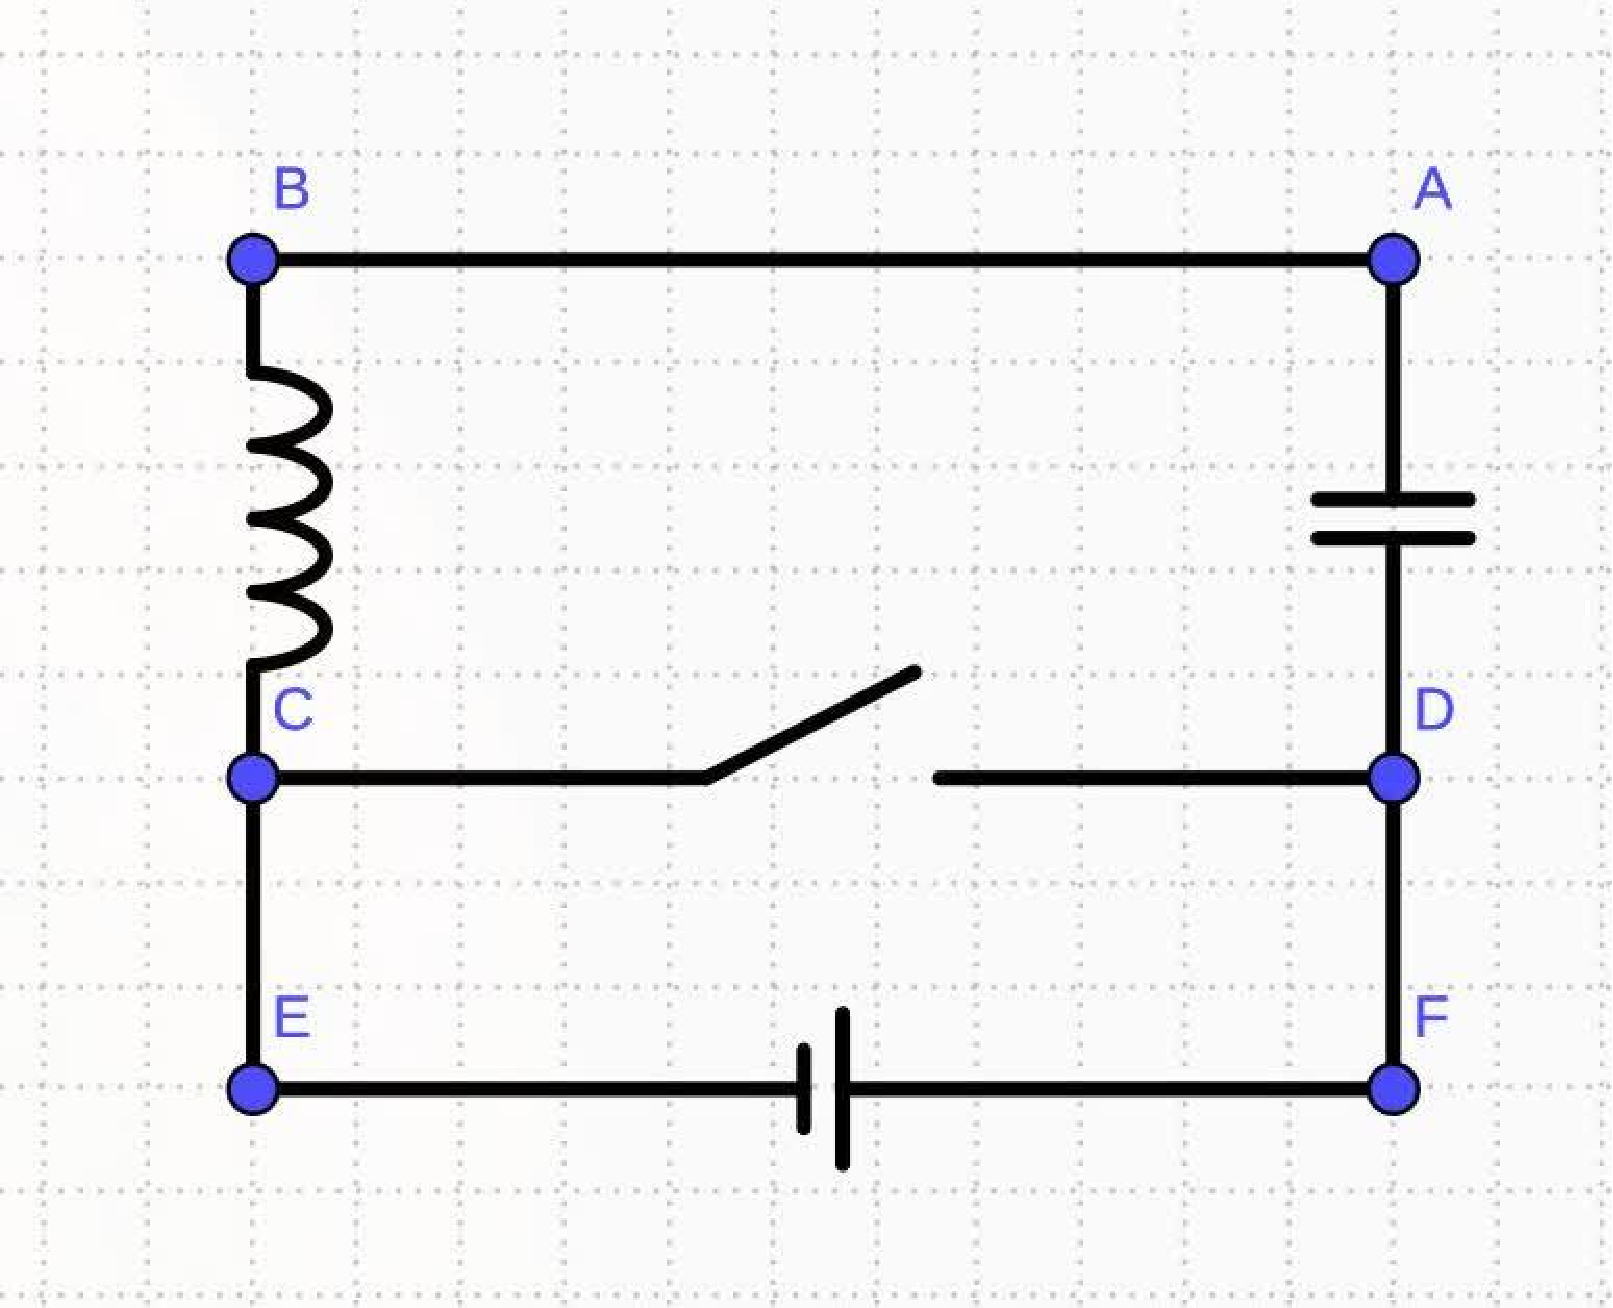
\includegraphics[width=0.8\textwidth]{schaltplan-einzelschwingkreis.pdf}
    \caption{Aufbau der Schwingkreise}
\end{figure}
\begin{figure}[H]
    \centering
    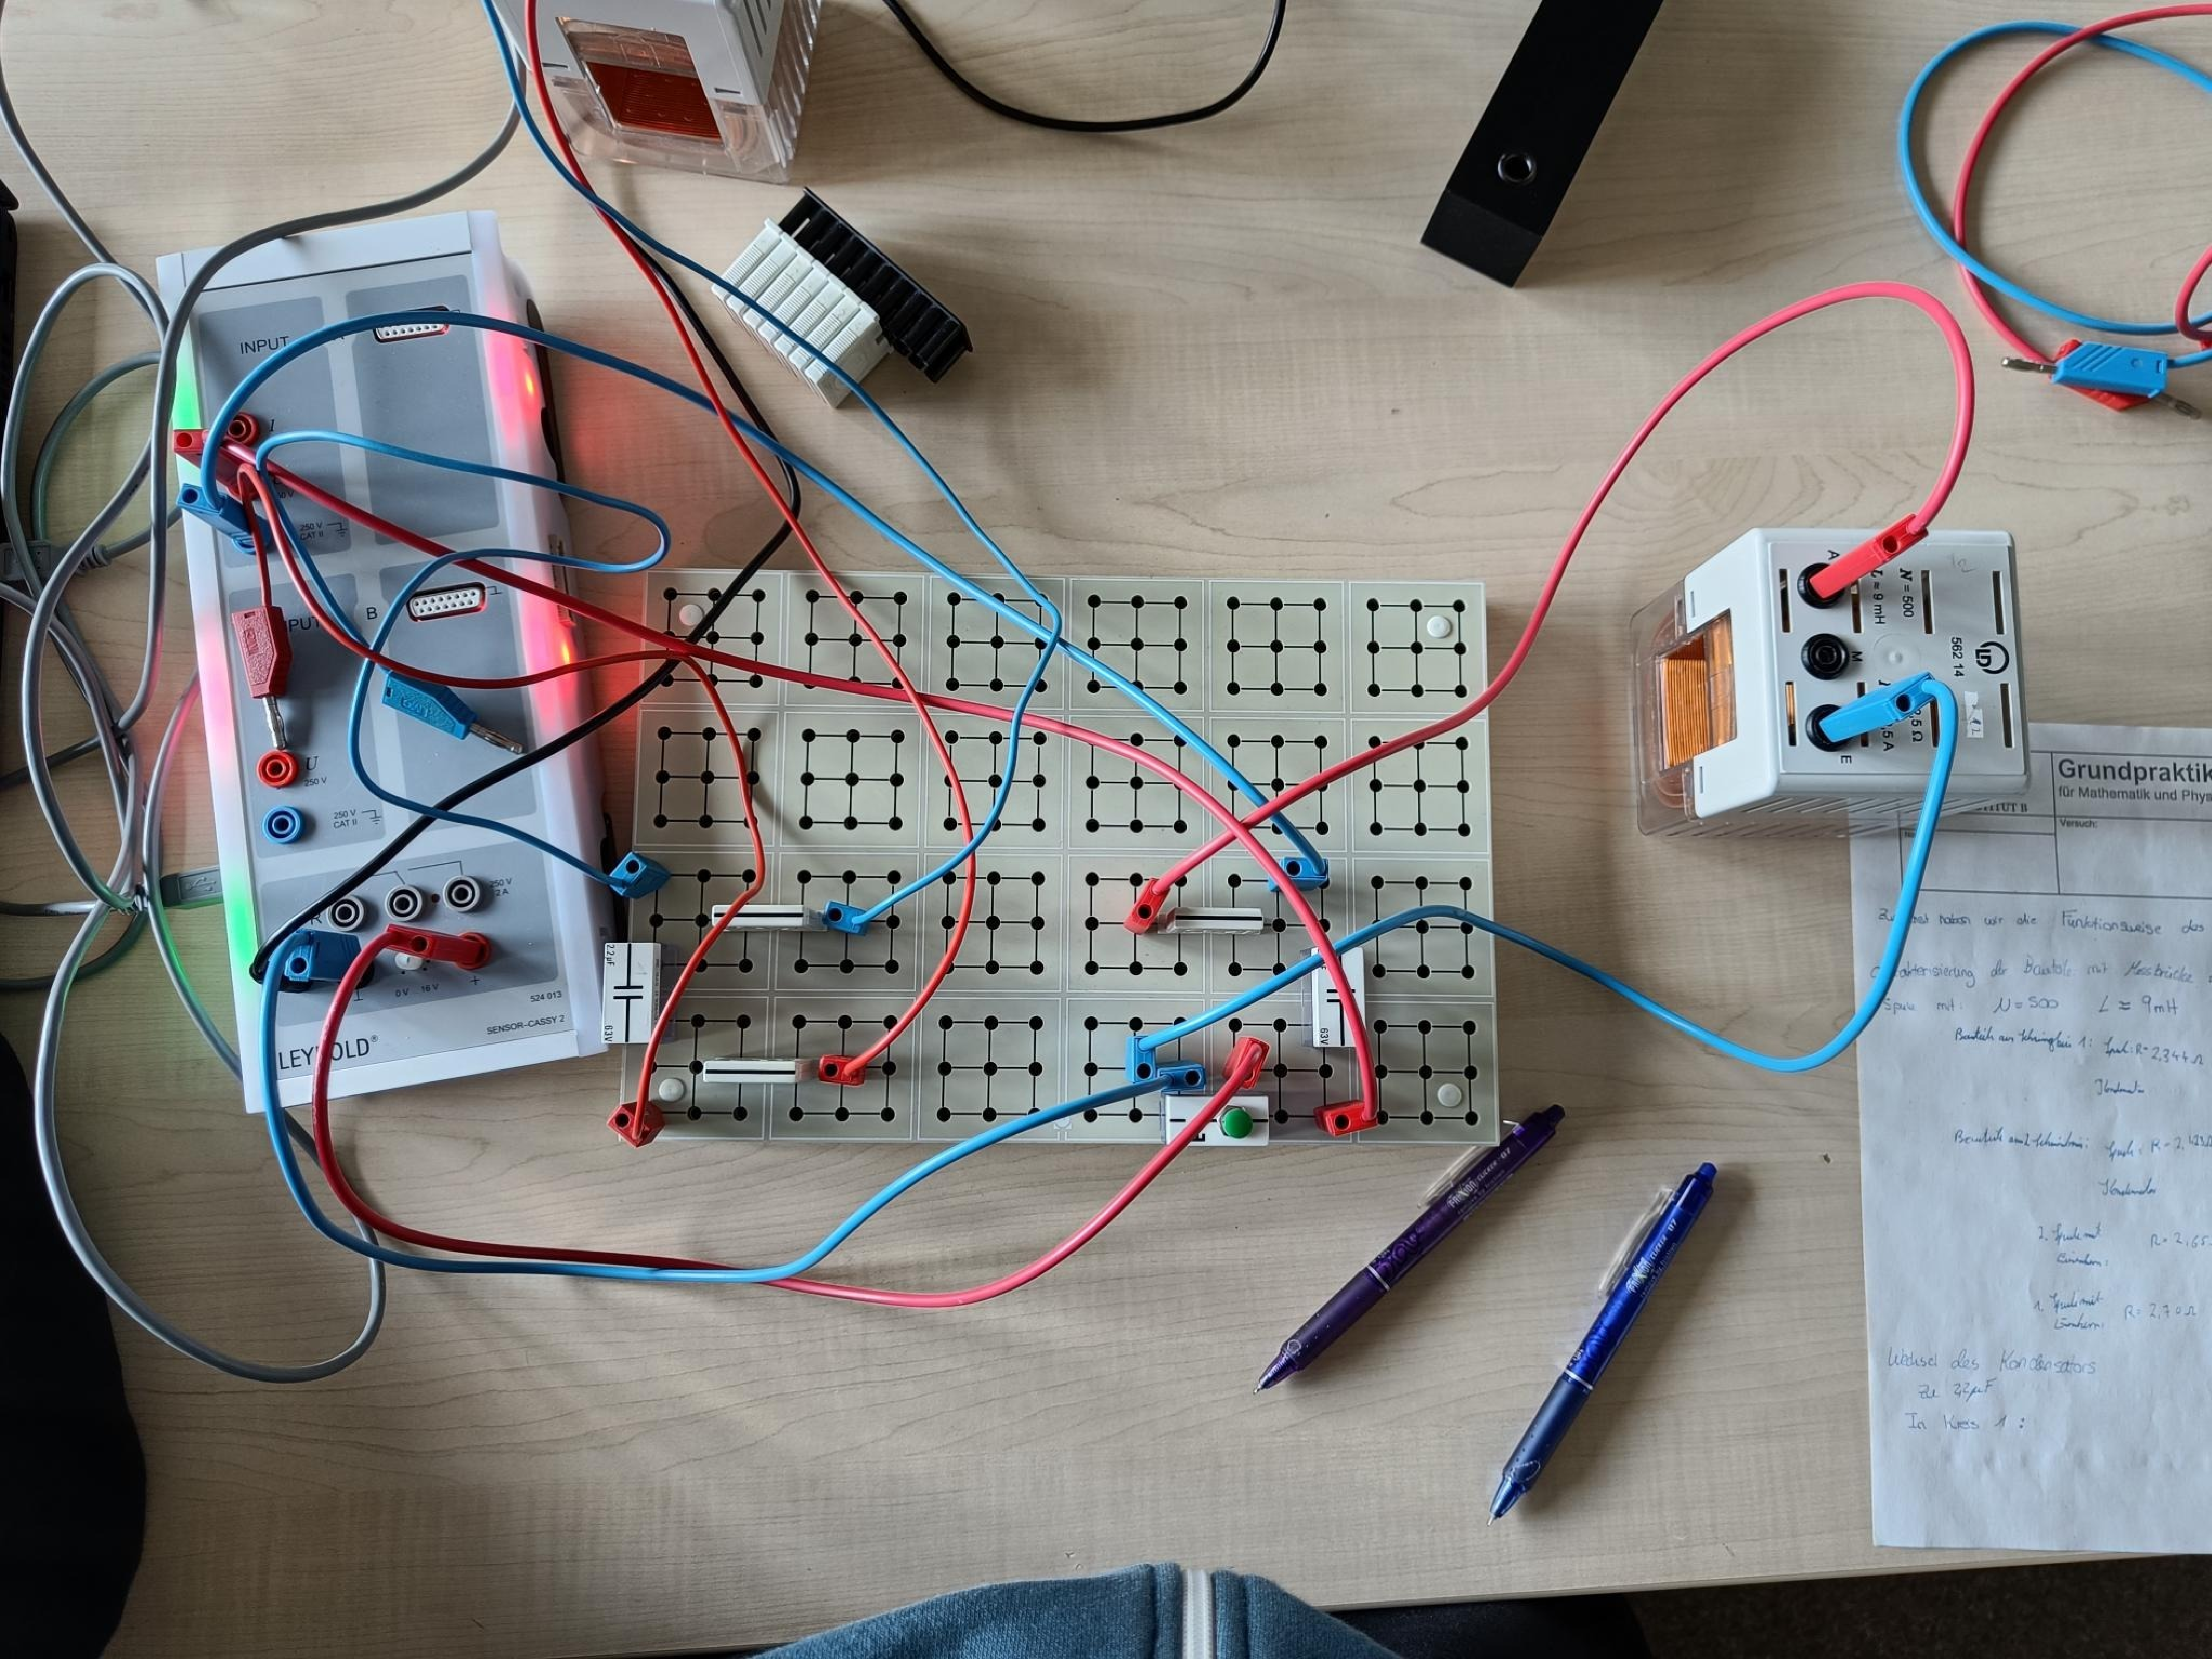
\includegraphics[width=0.8\textwidth]{bilder/schwingkreis2.pdf}
    \caption{Aufbau der beiden Schwingkreise}
\end{figure}

Oben ist ein Bild von beiden Schwingkreisen zu sehen, wobei links der 1. ist und rechts der 2.
Hier wird der 2. Schwingkreis vermessen, weshalb der 1. Schwingkreis auch nicht eingesteckt machen im CASSY.
 
Zudem haben wir mit Spule zwei und Kondensator zwei einen zweiten Schwingkreis aufgebaut.
Der Aufbau und die Schaltskizze des zweiten Schwingkreises ist gleich zu dem des ersten.
Insgesamt hatten wir 2 getrennte Schwingkreise, aber nur einen Schalter und eine Spannungsquelle (da wir die Schwingkreise später koppeln werden).
Deshalb haben wir die Spannungsquelle und den Schalter dann jeweils umgesteckt, um die zwei Schwingkreise getrennt zu messen.




\subsection{Durchführung}
Zuerst haben wir eine Spannung von $U_0 = 6.2V$ angelegt da bei dieser Spannung die Maximale Stromstärke der Spule ( $2.5A$ ) nicht überschritten wird.
Also haben wir als Spannungsbereich des CASSY-10V bis 10V eingestellt.
Anschließend haben wir ein paar Testmessungen gemacht, um die optimalen Messeinstellungen zu finden.
Diese Testmessungen haben wir jedoch noch mit unserer 'alten' Kapazität gemacht ( $C = 10 \mu F$ ).
Beim einbauen der neuen haben wir die Messparameter aber angepasst.\\
Dafür haben wir die Periodendauer ohne Widerstand genähert (da dieser für eine grobe Abschätzung vernachlässigbar klein ist).
\begin{equation}
    T = 2 \pi \sqrt{LC} = 2 \pi \sqrt{9mH \cdot 2.2 \mu F} = 884 \mu s
\end{equation}
Nach dem Nequisst Theorem muss die Abtastrate mindestens doppelt so groß sein wie die Frequenz.
Um eine ausreichende Auflösung des Fourier Peaks zu haben, und da diese Messung nur eine Abschätzung war, haben wir $ 50 \mu s $ als Messintervall gewählt, da dieses mehr als das 10x ist.

 
Die Schwingung im Schwingkreis startet in dem Moment, in dem man den Taster drückt, und sich der Kondensator anfängt zu entladen, da soll auch die Messung starten.
Damit der Schwingkreis ungestört schwingen kann, muss der Taster auch während der gesamten Messung gedrückt bleiben.
Entsprechend haben wir den Trigger vom Cassy auf 6.1V fallende Flanke gestellt um die Messung zu starten.
Dabei haben wir 6.1V gewählt, da so noch der Großteil der ersten Schwingungsperiode mit aufgezeichnet wird.
0.1V Abstand sind genug um Störeffekte vom schließen des Schalters nicht auf zu zeichnen.
Den zweiten Schwingkreis haben wir dabei 10 mal vermessen, um die Statistische Unsicherheit auf die Frequenz zu bestimmen.

Den ersten Schwingkreis haben wir dabei nur einmal vermessen, da wir davon ausgehen können, das die Statistische Unsicherheit bei beiden Schwingkreisen gleich ist, da wir den gleichen Aufbau verwendet haben und auch sonst gleiche Messbedingungen hatten.



Nachdem die Messung beendet ist, wir das Frequenz Spektrum mit hilfe einer Fouriertransformation analysiert.
Die Länge der Messung beeinflusst dabei die Auflösung der Fouriertransformation.
 
\begin{figure}[H]
    \centering
    \includegraphics[width=0.8\textwidth]{plots/schwingkreis-alt-test-200us-0.01s_fft_zoom.pdf}
    \caption{Zoomin Plot der FFT der Testmessung mit Messdauer = 0.01s}
\end{figure}
Wie zu sehen ist bei diese Testmessung, ist das Fourierspektrum nur auf $ \pm 10Hz $ genau. Das bedeutet das die Messdauer von 0.01s zu kurz ist.
Als Messdauer haben wir später 0.5s Sekunden gewählt, da wir dann eine zufridenstellende (Weniger als 1\%) Auflösung hatten.

Hier eine übersicht der Messeinstellungen. Dabei haben wir den Kanal auf den getriggert wird immer auf den gestellt, an welchem der zu messende Schwingkreis angeschlossen war.
\begin{table}[H]
        \centering
        \begin{tabularx}{1\textwidth}{X X X X} % adjust width as needed
            \toprule
            \textbf{Intervall} & \textbf{Messzeit} & \textbf{Trigger} & \textbf{Messbereich (für beide Eingäge)} \\
            \midrule
            200$\mu$s  & 0.5s & 6.1V fallend & -10V - 10V \\
            \bottomrule
        \end{tabularx}
        \caption{Messwertserfassungseinstellungen des CASSY}
        \label{tab:mytable}
    \end{table}
     
Anschließend haben wir noch zwei Rauschmessung gemacht: einmal mit geöffnetem und einmal mit geschlossenem Schalter nach dem Schwingvorgang.
Diese haben wir gemacht, um daraus Offsets zu berechnen um unsere Messung des Wiederstandes zu präzisieren.


\subsubsection{Rohdaten}

Insgesamt hatten wir also die Kondenstorspannung beim Schwingungsvorgang in zweiten Schwingkreis 10x gemessen. Und im ersten Schwingkreis ein mal. 
So wie eine Rauschmessung bei 0V und bei ca. 6V. 

\begin{figure}[H]
    \centering
    \includegraphics[width=1\textwidth]{plots/schwingkreis_2_01.pdf}
    \caption{Schwingungsverlauf im zweiten Schwingkreis}
\end{figure}


\begin{figure}[H]
    \centering
    \includegraphics[width=1\textwidth]{plots/schwingkreise_zoom.pdf}
    \caption{Schwingungsverlauf der beiden Schwingkreis zoom-in}
\end{figure}

Oben können sie Exemplarisch einen Schwingungsverlauf im zweiten Schwingkreis sehen. 
Das obere Bild zeigt die Messung über die gesamte Messdauer. 
Sehr gut kann hier der Exponentielle Abfall der Amplitude erkannt werden. Bereits nach ca. 0.03s ist die Amplitude auf null abgefallen. 
Das Messen des großen Zeitintervalls ergibt sin, dass dies die Auflösung bei der FFT erhöht.


Im zweiten Plot, kann ein Zoom-in der Schwingung gesehen werden.  Hier können wir sehr gut sehen, dass die Schwingung einem Kosinus förmigen Verlauf entspricht.

Die Amplitude fällt nach Augenmaß Exponentiell ab.

Zu diesen Schwingungsverläufen haben wir, jeweils eine FFT gemacht, um zu überprüfen, ob die Frequenz des Schwingkreis aus der Messung gut bestimmbar ist.


\begin{figure}[H]
    \centering
    \includegraphics[width=1\textwidth]{plots/schwingkreis_2_01_fft_complete.pdf}
    \caption{Schwingungsverlauf im ersten Schwingkreis}
\end{figure}


\begin{figure}[H]
    \centering
    \includegraphics[width=1\textwidth]{plots/schwingkreis_2_01_fft_small_zoom.pdf}
    \caption{Schwingungsverlauf im ersten Schwingkreis zoom-in}
\end{figure}

Zu sehen ist, dass wir einen klaren peak bei einer bestimmten Frequenz haben, es sind keine Frequenzen von anderen Schwingungen zu sehen. 
Dies war aus den Kosinus förmigen Verlauf der Messung zu erwarten.
Im unteren Graphen ist ein Zoom-in der FFT zu sehen, hier kann man gut erkennen, dass wir eine klare Spitze haben. 
Die Frequenz des Schwingkreis kann später durch weiteres zoomen festgestellt werden.

hier noch die Schwingungsverläufe von unserem Ersten Schwingkreis. Diese sind Augenscheinlich sehr ähnlich zu den des zweiten.
Dies ist auch zu erwarten, da wir gleich Bauteil verwendet haben.

\begin{figure}[H]
    \centering
    \includegraphics[width=1\textwidth]{plots/schwingkreis_1_01.pdf}
    \caption{Schwingungsverlauf im ersten Schwingkreis}
\end{figure}


\subsection{Auswertung}
Da wir die Frequenz der Schwingkreise bestimmen sollten, haben wir uns die FFT im Bereich des Peaks genauer angesehen.
\begin{figure}[H]
    \centering
    \includegraphics[width=1\textwidth]{plots/schwingkreis_1_01_fft_zoom.pdf}
    \caption{FFT Zoom vom ersten Schwinkgreis um den Peak mit eingezeichnetem Peak}
\end{figure}

Auch zu dieser Messung haben wir eine FFT gemacht welche Augenscheinlich eine sehr ähnliche Peakfrequenz aufweist wie die des zweiten Schwingkreis.

\begin{figure}[H]
    \centering
    \includegraphics[width=1\textwidth]{plots/schwingkreis_1_01_fft_complete.pdf}
    \caption{Schwingungsverlauf im ersten Schwingkreis}
\end{figure}

In diesem Zoom-in können wir erkennen, dass die Peakfrequenz leicht von der des Zweiten Schwingkreises abweichen wird.

\begin{figure}[H]
    \centering
    \includegraphics[width=1\textwidth]{plots/schwingkreis_1_01_fft_small_zoom.pdf}
    \caption{Schwingungsverlauf im ersten Schwingkreis zoom-in}
\end{figure}




\begin{aufgabe}{Gekoppelte Schwingung: Schwebung}
  Stellen Sie für einen festen Kopplungsgrad $k$ eine Schwebung
  dar. Zeigen Sie jeweils die Fourierspektren, bestimmen Sie die
  Eigenfrequenzen und daraus den Kopplungsgrad sowie dessen
  Messunsicherheit. Bestimmen Sie die zeitliche Verschiebung
  $\Delta{}t$ zwischen den beiden Einhüllenden der Schwebungen der
  beiden Kondensatoren und vergleichen Sie sie mit Ihrer
  Erwartung. Stellen Sie dar, wie sich das Frequenzspektrum mit dem
  Abstand der Spulen ändert. Untersuchen Sie die Verstärkung der
  Kopplung durch Verwendung eines Eisenkerns in den beiden Spulen.
\end{aufgabe}

in diesem Versuchsteil wollen wir nun die gekoppelten Schwingkreise auf ihre Frequenz untersuchen. Wobei hier nur einer der beiden Kondensatoren aufgeladen wird.
Hierfür haben wir zunächst die zwei Spulen ohne Abstand nebeneinander gestellt (jeweils mit dem Loch zueinander). 
Außerdem haben wir die Spannung am zweiten Kondensator gemessen, indem wir das Sensor CASSY parallel zu diesem geschallten haben. 
Die Schaltung kann dem Schaltbild unten entnommen werden. \\



\subparagraph{Gekoppelte Schwingung: Schwebung}

%TODO : Schaltbild einfügen

Wenn nun Spannung angelegt wird, wird der Kondensator in Schwingkreis 1 aufgeladen. 
Erst durch drücken des Tasters wird dieser Schwingkreis geschlossen und die Schwingung startet. 
Durch die Kopplung über die Spulen wird so auch der zweite Schwingkreis zur Schwingung angeregt.
Für den gekoppelten Schwingkreise haben wir die selben Messwerterfassungseinstellungen wie beim Messen der einzelnen Verwendet. 
So ist unsere Messung wieder durch einen Triger 6.1V Fallende Flanke auf Schwingkreis 1 gestartet.

Um eine Messung auf zu nehmen wird der Kondensator in Schwingkreis 1 zunächst geladen.
Durch drücken des Tasters wird die Spannungsquelle kurzgeschlossen, und der Schwingkreis 1 geschlossen. In diesem beginnt der Schwingungsvorgang.
Über die Kopplung der Spulen wird der zweite Schwingkreis ebenfalls zur Schwingung angeregt. An beiden Schwingkreisen messen wir den Spannungsverlauf am Kondensator. 
Bei diesem konnten wir gut den Schwingungsverlauf des gekoppelten Schwingkreis sehen, als auch die Schwebung. 
Von beiden haben wir eine FFT gemacht, um daraus die Fundamentalschwingungen des Schwingkreises zu bestimmen welche sich als zwei Peaks im Graph der FFT gezeigt haben.\\ 

Zur Bestimmung des Einfluss des Abstands auf den Kopplungsgrad haben wir die Spulen in 0.5cm schritten auseinander bewegt. 
Bei jedem dieser schritte haben wir eine Messung wie oben durchgeführt. Dabei haben wir jedes mal uns die FFT der beiden Schwingkreise angeschaut, um zu schauen ab welchem Abstand die Peaks bei der FFT nicht mehr zu trennen sind. Durch Vergrößerung des Abstands sind die Peaks näher zusammen gerückt.
Ab 3cm Abstand waren diese nicht mehr zu trennen.

%TODO : Bild vom Abstand der Spulen einfügen

Dabei ist uns aufgefallen, dass in Schwingkreis 1 die zwei Fundamentalfrequenzen länger trennbar sind als im zweiten. 

Zuletzt haben wir in die zwei Spulen auf einen gemeinsamen Eisenkern geschoben, um die Kopplung so zu erhöhen. Mit dieser Konfiguration haben wir die Messung noch mal durchgeführt. 

\subsubsection{Rohdaten}

Insgesamt haben wir in diesem Versuchsteil also 9 Messungen durchgeführt, 8 Messungen mit verschiedenen Abständen und eine Messung mit dem Eisenkern. 


\begin{aufgabe}{Gekoppelte Schwingung: gleich- und gegensinnige Anregung}
  Stellen Sie für einen festen Kopplungsgrad $k$ nacheinander die
  beiden Fundamentalschwingungen dar. Zeigen Sie jeweils die
  Fourierspektren und bestimmen Sie die zugängliche
  Eigenfrequenz. Berechnen Sie den Kopplungsgrad sowie dessen
  Messunsicherheit. Vergleichen Sie mit den Werten aus der Schwebung.
\end{aufgabe}
   
   
\end{document}

%TODO : Peak Linie aus Rohdaten raus nehmen
%TODO : Peak beschriften